\documentclass[openany,12pt,a4paper]{report}
\usepackage{subfiles}
\usepackage[numberedsection]{glossaries}
\usepackage[]{graphicx}
\usepackage{float}
\usepackage{multirow}
\graphicspath{{./img/}{./../img/}}
\usepackage{../StileDoc}
\title{Manuale Utente}
\author{}

%Ultima versione documento
\newcommand{\versione}{0.2.0}

% Stile per il glossario
\newglossarystyle{glossaryStyle}{
	\setglossarystyle{altlistgroup}
	\renewcommand*{\glsgroupheading}[1]{
		% Tolgo la numerazione per l'indice
		\setcounter{secnumdepth}{0}
		\section{##1}
		\vspace*{-\baselineskip}
		% Solo per fare un po' di spazio tra la lettera e le voci
		\item\makebox[\linewidth]{\hspace*{2cm}}
	}
}

\glsaddall

\makeglossaries

%Term definitions
\newglossaryentry{Speect}{name=Speect, description={Libreria di Text-To-Speech di riferimento per il progetto DeSpeect}}
\newglossaryentry{GCC}{name=GCC, description={Compilatore C++ di riferimento per il progetto DeSpeect}}
\newglossaryentry{GitHub}{name=GitHub, description={Servizio di versionamento per progetti software}}
\newglossaryentry{Qt}{name=Qt, description={Libreria multipiattaforma per lo sviluppo di programmi con interfaccia grafica tramite l'uso di widget}}
\newglossaryentry{utterance}{name={Utterance}, description={La più piccola unità del discorso, una parte di esso che inizia e termina con una pausa chiara}}
\newglossaryentry{relation}{name={Relation}, description={Rappresenta una struttura come una parola, sillaba, fonema o anche un obiettivo di durata e gli item sono il contenuto di questa struttura.}}
\newglossaryentry{framework}{name={Framework}, description={Piattaforma che funge da strato intermedio tra un sistema operativo e il software che lo utilizza.}}
\newglossaryentry{issue}{name={Issue}, description={Unità di lavoro per realizzare un miglioramento in un sistema. Un issue potrebbe essere un bug, una funzionalità richiesta, attività, documentazione mancante e così via.}}


\begin{document}
	\makeatletter
	\begin{titlepage}
		\setlength{\headsep}{0pt}  
		\begin{center}
			
\includegraphics[width=0.5\linewidth]{img/logo.png}\\[1em]
			{\huge \bfseries  \@title }\\[10ex]
			\textbf{\Large Informazioni Documento} \\[2em]
			\bgroup
			\def\arraystretch{1.5}
			\begin{tabular}{l|l}
				\textbf{Versione} & \versione{} \\
				\textbf{Responsabile} & Marco Focchiatti\\
				\textbf{Redattori} &  Manfredi Smaniotto, Marco Focchiatti,\\
				& Cristiano Tessarolo, Giulio Rossetti \\
				\textbf{Verificatori} & Manfredi Smaniotto, Marco Focchiatti \\
				\textbf{Distribuzione} & Prof. Tullio Vardanega \\
				& Prof. Riccardo Cardin \\
				& Mivoq S.R.L. \\
				& Gruppo Graphite \\
				\textbf{Uso} & Esterno \\
				\textbf{Recapito} & graphite.swe@gmail.com \\
			\end{tabular}
			\egroup
		\end{center}
	\end{titlepage}
	\makeatother
	
	\thispagestyle{empty}
	\newpage
	
	%REGISTRO DELLE MODIFICHE
	
	\chapter*{Registro delle modifiche}
	\setlength\LTleft{-22mm}
	\begin{longtable}{|p{20mm}|p{20mm}|p{40mm}|p{30mm}|p{50mm}|}
		\hline
		\textbf{Versione} & \textbf{Data} & \textbf{Autore} & \textbf{Ruolo} & \textbf{Descrizione} \\
		
		\hline 0.2.0 & 2018-04-15 & - & Verificatore & Verifica da §5 a §8 e appendici \\
		\hline 0.1.4 & 2018-04-14 & - & Amministratore & Stesura appendici \\
		\hline 0.1.3 & 2018-04-13 & - & Amministratore & Stesura §8 \\
		\hline 0.1.2 & 2018-04-12 & - & Progettista & Stesura §7 §3 \\		
		\hline 0.1.1 & 2018-04-12 & - & Progettista & Stesura §5 - §6 \\
		\hline 0.1.0 & 2018-04-11 & - & Verificatore & Verifica da §1 a §4 \\
		\hline 0.0.5 & 2018-04-08 & - & Amministratore & Stesura §4 \\	
		\hline 0.0.4 & 2018-04-08 & - & Amministratore & Stesura §3 \\
		\hline 0.0.3 & 2018-04-07 & - & Amministratore & Stesura §2 \\
		\hline 0.0.2 & 2018-04-06 & - & Amministratore & Stesura §1 \\
		\hline 0.0.1 & 2018-04-05 & - & Amministratore & Creata struttura documento \\
		\hline
		
	\end{longtable}
	
	% INDICE
	\tableofcontents
	
	% INTRODUZIONE
	
	\chapter{Introduzione}
	
	\section{Scopo del documento}
	
	Il documento ha la finalità di illustrare, a coloro che volessero interfacciarsi con l’applicazione
	\textit{"DeSpeect: un'interfaccia grafica per Speect"}, i requisiti necessari per poterlo utilizzare e le modalità di installazione e di utilizzo. 
	Nonostante la versione attuale rappresenti una prima bozza del documento, una volta concluso esso rappresenterà sia una guida che un riferimento completo per l’utilizzo del prodotto da parte di un utente.
	
	\section{Scopo del prodotto}
	
	Lo scopo del progetto è la realizzazione di un’interfaccia grafica per \glossario{Speect}{Speect} [Meraka Institute(2008-2013)], una libreria per la creazione di sistemi di sintesi vocale, che agevoli l’ispezione del suo stato interno durante il funzionamento e la scrittura di test per le sue funzionalità.
	
	\section{Informazioni utili}
	
	La stesura di questo documento assume come utente target del prodotto un programmatore esperto nell'utilizzo di \textit{Speect} e dei linguaggi di programmazione C e C++. \\
	\noindent Per completezza, viene riportato in appendice §A un glossario comprensivo di termini tecnici o riguardanti particolari funzionalità di \textit{DeSpeect}. Per identificare i termini presenti nel glossario, la loro prima occorrenza all’interno del documento è riportata in corsivo e marcata con una G al pedice. 
	
	%quando caricheremo su github in una repository apposita il manuale sviluppatore
	\begin{comment}
	\\ \noindent Per i manutentori del prodotto o per chi fosse interessato alla sua integrazione/incremento, può invece consultare il manuale sviluppatore reperibile all'indirizzo: \url{...}
	\end{comment}
	
	\section{Riferimenti informativi}

	\begin{itemize}
		\item \textbf{Documentazione Speect:} \\
		\url{http://speect.sourceforge.net/contents.html};
		\subitem Documentazione ufficiale della libreria di \textit{Text-To-Speech} di riferimento per il progetto.
		
		\item \textbf{Documentazione Qt:} \\
		\url{http://doc.qt.io/};
		\subitem Documentazione ufficiale del \glossario{framework}{framework} utilizzato per lo sviluppo dell'interfaccia grafica.
		
		\item \textbf{Documentazione CMake:} \\
		\url{https://cmake.org/documentation/}.
		\subitem Documentazione ufficiale del framework utilizzato per la build del prodotto. 
	\end{itemize}

	\chapter{Requisiti di sistema}
	
	L'installazione ed esecuzione del software DeSpeect richiede i seguenti prerequisiti:
	
	\begin{itemize}
		\item Sistema operativo Unix / Unix-like (il software è stato testato solo per piattaforma Ubuntu 16.04 LTS)
		\subitem \url{https://www.ubuntu.com/download/desktop}
		\item CMake (versione minima 2.8)
		\subitem \url{https://cmake.org/download/}
		\item Compilatore ANSI C/ISO C90 \glossario{GCC}{GCC} (versione minima 5.0)
		\subitem \url{https://gcc.gnu.org/install/binaries.html}
		\item \glossario{Qt}{Qt} 5.9.0
		\subitem \url{https://www.qt.io/download}
		\item Git
		\subitem \url{https://git-scm.com/} 
		\item Curl 
		\subitem \url{https://curl.haxx.se/}
		\item Swig 
		\subitem \url{http://www.swig.org/}
		\item libxml2-dev
		\subitem \url{https://packages.debian.org/stretch/libxml2-dev} 
		\item python-dev
		\subitem \url{https://pypi.python.org/pypi/dev/0.4.0}
	\end{itemize}	
	 
	\chapter{Installazione e configurazione} 
	
	DeSpeect è reperibile su GitHub al seguente link:
	\begin{center}
		\url{https://github.com/graphiteSWE/DeSpeect}
	\end{center}
	
	\noindent Una volta soddisfatti i prerequisiti descritti in §2 "Requisiti di sistema" di questo documento, per installare ed eseguire il software è necessario seguire la seguente procedura:
	\begin{enumerate}
		\item Clonare o scaricare il repository sulla propria macchina;
		\item Entrare nella cartella scaricata ed eseguire lo script \verb|build.sh| presente al suo interno. Tale script installerà Speect ed effettuerà una build del progetto all'interno nella directory \verb|DeSpeect/build/|.
		\item Per eseguire DeSpeect, entrare nella directory \verb|DeSpeect/build/| ed eseguire il comando \verb|./main|.
	\end{enumerate}
	
	\chapter{Guida all'utilizzo}
	Viene di seguito illustrata la guida all'utilizzo del software DeSpeect. \\
	Si fa notare che i termini evidenziati in \textit{corsivo} corrispondono a pulsanti specifici presenti all'interno dell'applicazione.
	
	\section{Interfaccia grafica}
	
	\begin{figure}[H]
		
		\centering
		
		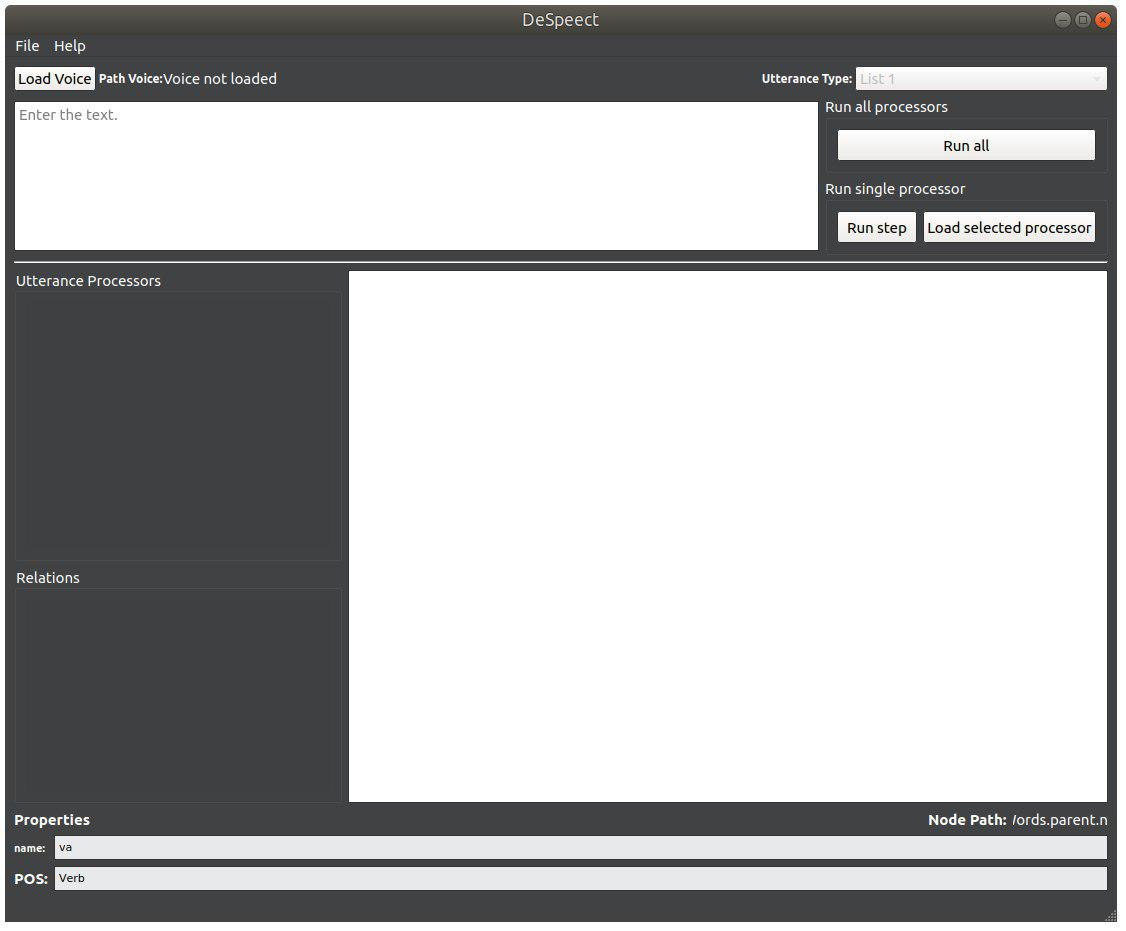
\includegraphics[scale=0.45]{./img/avvio}
		
		\caption{Interfaccia grafica - Schermata iniziale}
	
	\end{figure}

	All'avvio dell'applicazione viene presentata la schermata riportata in Figura 4.1. L'interfaccia grafica è costituita dalle componenti illustrate nelle sezioni seguenti:
 	
 	\subsection{Menù dell'applicazione}
 	Menù situato nella parte superiore della schermata. Tramite il menù \textit{File} è possibile interagire con alcune funzionalità offerte dal sistema, mentre tramite il menù \textit{Help} è possibile visualizzare manuale utente e licenza del prodotto (vedi Figura 4.2). Il menù è sempre disponibile in qualunque posizione all'interno dell'applicazione e al suo interno è possibile selezionare le seguenti voci:
 	
 	\subsubsection{File} 
 		\begin{itemize}
 			\item \textbf{Save Voice JSon}: salva il file JSon;
 			\item \textbf{Load HRG Graph}: carica un grafo HRG;
 			\item \textbf{Save HRG Graph}: salva un grafo HRG;
 			\item \textbf{Save Audio file}: salva il file audio prodotto in seguito all'esecuzione di \textit{Speect};
 			\item \textbf{Search from path}: cerca un nodo inserendo come input un percorso specifico (es. Words.parent.n);
 			\item \textbf{Exit}: chiude l'interfaccia \textit{DeSpeect}.
 		\end{itemize}
 		
 		\begin{figure}[H]
 			
 			\centering
 			
 			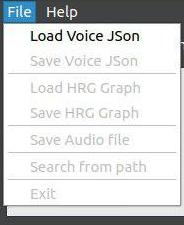
\includegraphics[width=.4\textwidth]{./img/menu_file}
 			
 			\caption{Menù dell'applicazione - Sezione "File"}
 			
 		\end{figure}
 	
 	\subsubsection{Help}
 		\begin{itemize}
 			\item \textbf{Manual}: apre il manuale utente;
 			\item \textbf{Licence}: visualizza la licenza di \textit{DeSpeect}.
 		\end{itemize}
 		\begin{figure}[H]
 			
 			\centering
 			
 			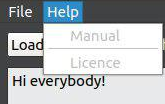
\includegraphics[width=.4\textwidth]{./img/menu_help}
 			
 			\caption{Menù dell'applicazione - Sezione "Help"}
 			
 		\end{figure}
 	
 	\subsection{Pannello di configurazione}
 	Situato nella parte superiore della schermata sotto il menù citato al punto precedente. Qui è possibile caricare una voice (tramite pulsante \textit{Load Voice}), inserire input testuale (tramite area di testo dedicata), selezionare l'\glossario{utterance}{utterance} type e avviare l'esecuzione di \textit{Speect} eseguendo singolarmente ogni utterance processor (pulsante \textit{Run step}) o tutti assieme in sequenza (pulsante \textit{Run all}). Il pulsante \textit{Load selected processors}, infine, permette il caricamento della configurazione degli utterance processor selezionati tramite apposito pannello illustrato al punto successivo (vedi Figura 4.3);
 		\begin{figure}[H]
 			
 			\centering
 			
 			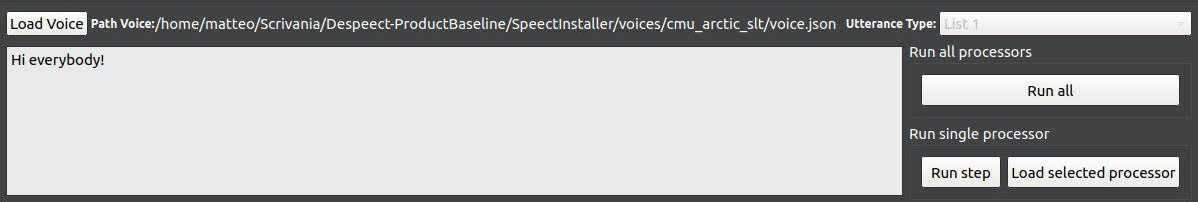
\includegraphics[width=\textwidth]{./img/pannello_configurazione}
 			
 			\caption{Interfaccia grafica - Pannello di configurazione}
 			
 		\end{figure}
 	
 	\subsection{Pannello degli utterance processor}
 	Situato sulla sinistra, sotto al pannello di configurazione. Qui è presente una lista degli utterance processor relativi alla voice caricata, a ognuno dei quali è assegnata una checkbox. Spuntando le checkbox l'utente seleziona gli utterance processor che desidera eseguire per un dato input tramite i pulsanti dedicati presenti nel pannello di configurazione (pulsanti \textit{Run all} e \textit{Run step}). Avviata l'esecuzione, i processor eseguiti verranno evidenziati dal colore verde, mentre quello corrente è riportato in grassetto (vedi Figura 4.4);
 		\begin{figure}[H]
 			
 			\centering
 			
 				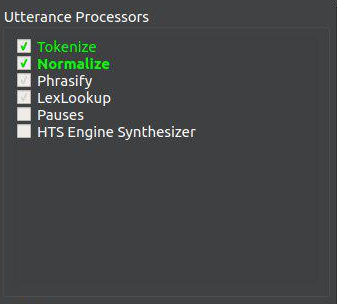
\includegraphics[width=.4\textwidth]{./img/pannello_processors}
 			
 			\caption{Interfaccia grafica - Pannello degli utterance processors}
 			
 		\end{figure}
 		
 	\subsection{Pannello delle relations}
 	Situato sulla sinistra, sotto al pannello degli utterance processor. Qui è possibile selezionare quali \glossario{relation}{relation} visualizzare nel grafo. Di default, il grafo mostra ogni relation disponibile, rimuovendo la spunta dalla checkbox della relation desiderata le componenti del grafo relative vengono rimosse dalla visualizzazione (vedi Figura 4.5);
 		\begin{figure}[H]
 			
 			\centering
 			
 				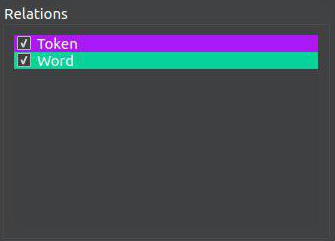
\includegraphics[width=.4\textwidth]{./img/pannello_relations}
 			
 			\caption{Interfaccia grafica - Pannello delle Relations}
 			
 		\end{figure}
 	
 	\subsection{Area del grafo}
 	Situata sulla destra, sotto al pannello di configurazione. Qui viene visualizzato il grafo relativo ad una data voice, input testuale e configurazione di utterance processor. I nodi sono selezionabili (nel cui caso, le informazioni relative al nodo vengono visualizzate nell'apposita barra approfondita al punto seguente) e spostabili (vedi Figura 4.6);
 		\begin{figure}[H]
 			
 			\centering
 			
 				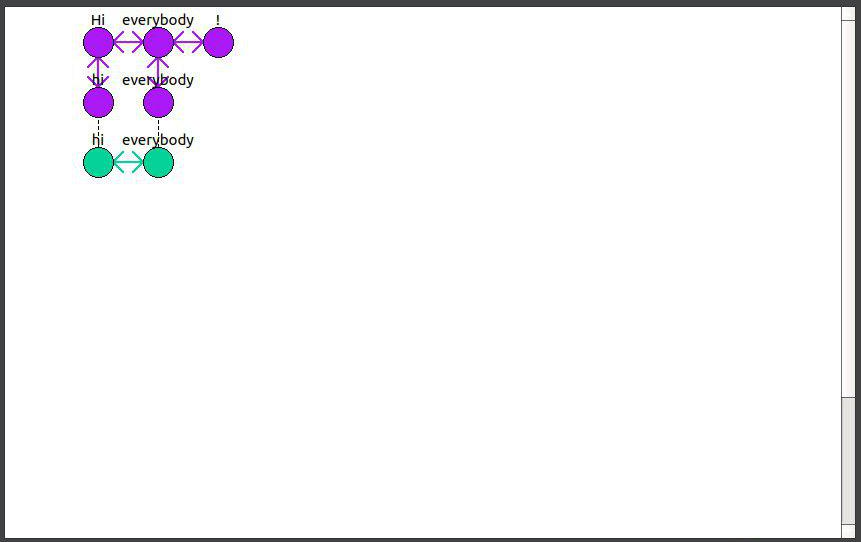
\includegraphics[width=\textwidth]{./img/area_grafo}
 			
 			\caption{Interfaccia grafica - Area del grafo}
 			
 		\end{figure}
 	
 	\subsection{Proprietà del nodo}
 	Situato nella parte inferiore dell'interfaccia. Qui vengono visualizzate le informazioni specifiche relative al nodo selezionato (vedi Figura 4.7).
 		\begin{figure}[H]
 			
 			\centering
 			
 				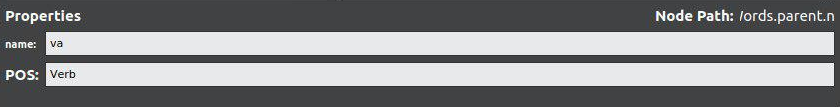
\includegraphics[width=\textwidth]{./img/proprieta_nodo}
 			
 			\caption{Interfaccia grafica - Proprietà del nodo}
 			
 		\end{figure}
	
	\section{Interagire con la voice}
	Questa sezione tratta dell'interazione con la voice (rappresentata da un file \verb|.json|), dal suo caricamento alla generazione dell'audio prodotto da \textit{Speect}.
	
	\subsection{Caricare la voice}
	Per caricare la voice è sufficiente cliccare il pulsante \textit{Load Voice}, situato nell'angolo in alto a sinistra del pannello di configurazione (vedi §4.1.2) o, in alternativa, cliccare sul menù \textit{File} e, successivamente, sulla voce \textit{Load Voice}.\\
	Una volta fatto ciò si aprirà il file browser del sistema operativo, che permetterà la ricerca di un file \verb|.json| corrispondente alla voice desiderata. Una volta reperito il file, sarà sufficiente aprirlo mediante file browser.\\
	A questo punto, se verrà visualizzato il percorso del file \verb|.json| subito dopo l'etichetta "Path Voice", vicino al pulsante di caricamento della voice, allora il caricamento della stessa avrà avuto successo.\\
	Nel caso in cui il caricamento del file abbia avuto esito negativo, è necessario ripetere la procedura assicurandosi si averla eseguita correttamente.
	
	\subsection{Generare l'audio relativo alla voice caricata}
	Successivamente al caricamento della voice, per generare l'audio relativo è sufficiente cliccare il pulsante \textit{Run all}. In questo modo verranno eseguiti gli utterance processor selezionati e visualizzato il grafo risultante, e \textit{Speect} genererà il file audio desiderato.\\
	Prima di procedere con l'esecuzione di \textit{Speect}, è possibile inserire un input testuale nell'apposita area di testo, nonché selezionare una diversa utterance type (nel caso fosse presente).
	
	\subsection{Salvare l'audio relativo alla voice}
	Uno volta eseguito \textit{Speect}, per salvare l'audio è sufficiente cliccare sul pulsante \textit{File} del menù e selezionare la voce \textit{Save Audio file}.\\
	Fatto ciò, si aprirà una finestra di ricerca del file browser dove cercare la cartella in cui salvare il file. Una volta trovata basterà selezionarla, cliccandoci sopra, scrivere il nome del file nella barra di testo dedicata e confermare.\\
	Il file audio prodotto avrà l'estensione \verb|.wav|.
	
	\section{Visualizzare il grafo}
	Per visualizzare il grafo è necessario aver caricato una voice, inserito un input testuale ed eseguito \textit{Speect} tramite pulsante \textit{Run all} o \textit{Run step}.\\
	Se sono state compiute tali azioni, viene visualizzato il grafo nell'area dedicata (§4.1.5), nonché la lista delle relation (§4.1.4).
	Il grafo è composto da:
	\begin{itemize}
		\item \textbf{Nodi}: visualizzati tramite cerchi con relativo name, i nodi hanno colori diversi a seconda della relazione a cui appartengono (la lista delle relation funge da legenda);
		\item \textbf{Archi}: visualizzati tramite frecce direzionali che collegano due nodi, anche gli archi sono di colori diversi a seconda della relazione a cui fanno riferimento.
	\end{itemize}
	
	\subsection{Visualizzare il grafo step-by-step}
	Eseguendo \textit{Speect} tramite pulsante \textit{Run step}, è possibile eseguire un utterance processor alla volta e vederne il risultato sul grafo, che ad ogni step si aggiorna aggiungendo nuove relazioni.
	
	\subsection{Visualizzare l'intero grafo}
	Eseguendo \textit{Speect} tramite pulsante \textit{Run all} è possibile eseguire tutti gli utterance processor in una sola volta e vedere subito il grafo completo.
	
	\section{Interagire con il grafo}
	Questa sezione spiega come poter interagire col grafo spostando nodi e archi, rimuovendo nodi e archi relativi a determinate relation dalla visualizzazione e come esportare il grafo.
	
	\subsection{Esportare il grafo generato}
	Per esportare un grafo è sufficiente cliccare \textit{File} dal menù e selezionare la voce \textit{Save HRG Graph}.\\
	Una volta fatto ciò, si aprirà una finestra di ricerca del file browser dove cercare la cartella in cui salvare il file. Una volta trovata basterà selezionarla, cliccandoci sopra, scrivere il nome del file nella barra di testo dedicata e confermare.
	
	\subsection{Importare il grafo}
	Per importare un grafo è sufficiente cliccare \textit{File} dal menù e selezionare la voce \textit{Load HRG Graph}.\\
	Una volta fatto ciò, si aprirà una finestra di ricerca del file browser dove cercare il file. Sarà dunque sufficiente reperirlo, selezionarlo e confermarne l'apertura.
	
	\subsection{Selezionare gli utterance processor}
	Nel pannello degli utterance processor (§4.1.3) è possibile interagire con i processor tramite le caselle di spunta a lato.\\
	Togliendo la spunta da un processor, esso non verrà eseguito da \textit{Speect}, e viceversa.
	
	\subsection{Interagire con le relation}
	Nel pannello delle relation è possibile interagire con esse tramite le caselle di spunta a lato.\\
	Togliendo la spunta da una relation, i relativi nodi verranno rimossi dalla visualizzazione del grafo, viceversa se si aggiunge la spunta, verranno aggiunti i relativi nodi al grafo.
	
	\subsection{Traslare elementi grafici}
	Questa sezione spiega come traslare gli elementi grafici che compongono il grafo, ovvero nodi e archi.
	
	\subsubsection{Traslare nodi}
	Per traslare un nodo è sufficiente cliccare su di esso tenendo premuto e, spostando il cursore, trascinarlo dove si desidera all'interno dell'area del grafo.
	
	\subsubsection{Traslare archi}
	Quando si trasla un nodo, gli archi che sono coinvolti direttamente con quel nodo si adatteranno alla nuova posizione del nodo.
	
	\chapter{Risoluzione dei problemi}
	
	\section{Errori in DeSpeect}
	In questa sezione viene fornito un elenco di tutti i possibili errori che si possono riscontrare utilizzando l’applicazione \textit{DeSpeect}.
	
	\subsection{Struttura dei codici di errore} 
	%Credo vada nelle norme di progetto
	
	\subsection{Log degli errori}
	
	\section{Problemi con il reperimento di Speect}
	
	\section{Segnalazione di bug}
	
	\textit{DeSpeect} potrebbe contenere bug o potrebbe essere desiderabile apportare modifiche e ampliamenti alle sue funzionalità. \\ È possibile segnalare malfunzionamenti o richieste di nuove funzionalità sotto forma di GitHub \glossario{issue}{issue} all’indirizzo:
	\begin{center}
		\url{https://github.com/graphiteSWE/DeSpeect}
	\end{center}
  oppure scrivendo direttamente all'indirizzo e-mail:
  \begin{center}
  	\url{graphite.swe@gmail.com}
  \end{center}
	
	\appendix
	
	\printglossary[style=glossaryStyle, nonumberlist]
	
\end{document}
